\documentclass[a4paper,12pt]{article}
\usepackage{graphicx}        % Képek beillesztéséhez szükséges csomag
\usepackage{lipsum}          % Zagyva szöveg generálására
\usepackage{caption}         % Feliratok beállítása
\usepackage{subcaption}      % Részábra környezethez
\usepackage[table]{xcolor}   % Színes táblázatokhoz
\usepackage{verbatim}        % Verbatim környezethez
\usepackage{listings}        % Programkód beillesztéséhez
\usepackage{float}           % Úszó elemek kezeléséhez
\usepackage{wrapfig}         % Szöveg körbefuttatása
\usepackage{multirow}        % Több soros cellák egyesítése táblázatban

\lstset{language=Python, tabsize=2, showtabs=false, showspaces=false, numbers=left, stepnumber=4, frame=single}

\begin{document}

\tableofcontents % Tartalomjegyzék
\listoffigures   % Ábrajegyzék
\listoftables    % Táblázatjegyzék

\newpage

\section{Ábrák feladat}

\subsection{a) Képek beillesztése csomaggal}
% 1a. feladat
Képbeillesztéshez a \texttt{graphicx} csomag szükséges, amelyet már a dokumentum elején betöltöttünk.

\subsection{b) Kép beillesztése max. 5 cm szélességgel és magassággal, torzítás nélkül}
% 1b. feladat
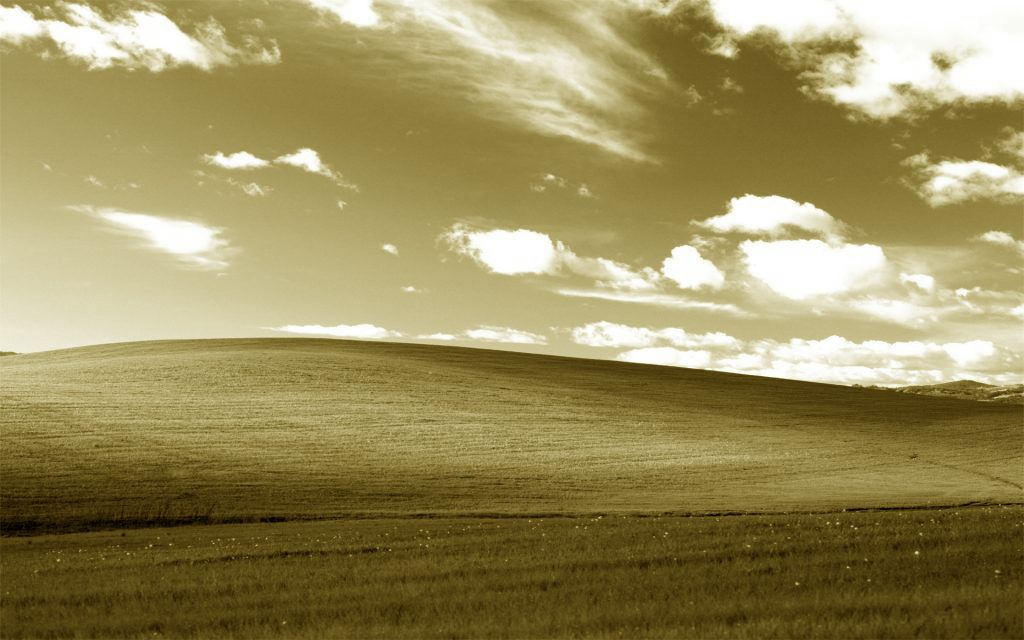
\includegraphics[width=5cm,height=5cm,keepaspectratio]{szepia.jpg}

\subsection{c) Kép úsztatás nélkül, szöveggel egy sorban}
% 1c. feladat
\lipsum[1] % Zagysor szöveg
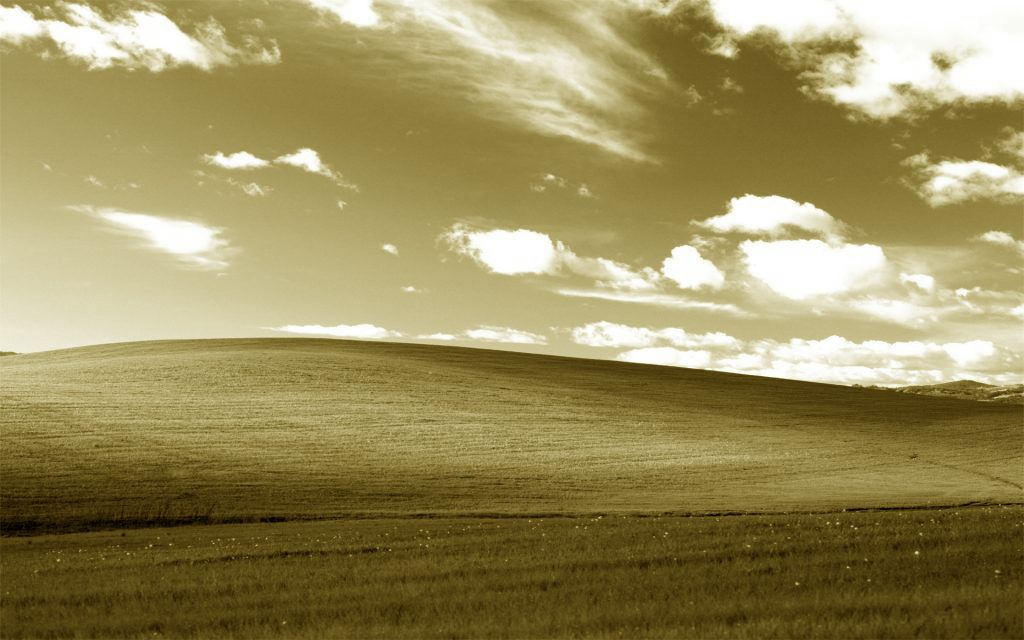
\includegraphics[width=5cm,height=5cm,keepaspectratio]{szepia.jpg}
\lipsum[2] % További zagysor szöveg

\subsection{d) Kép úszó ábra környezetben}
% 1d. feladat
\begin{figure}[h]
    \centering
    
\includegraphics[width=5cm,height=5cm,keepaspectratio]{szines.jpg}
    \caption{Úszó ábra példa}
    \label{fig:floating}
\end{figure}

\subsection{e) Transzformált kép beillesztése}
% 1e. feladat
\begin{figure}[h]
    \centering
    
\includegraphics[width=5cm,height=5cm,keepaspectratio,angle=45]{szines.jpg} % 45 fokos elforgatás
    \caption{Tükrözött kép}
    \label{fig:transformed}
\end{figure}

\subsection{f) Második felirat beillesztése (nem működik)}
% 1f. feladat
Az ábrákhoz csak egy felirat használható egyszerre, a második felirat hibát okozna:
% \caption{Második felirat (nem használható)}

\subsection{g) Ábrajegyzék listázása}
% 1g. feladat
Az ábrajegyzék a dokumentum elején automatikusan generálódott.

\subsection{h) Részábrák beillesztése}
% 1h. feladat
\begin{figure}[h]
    \centering
    \begin{subfigure}{0.45\textwidth}
        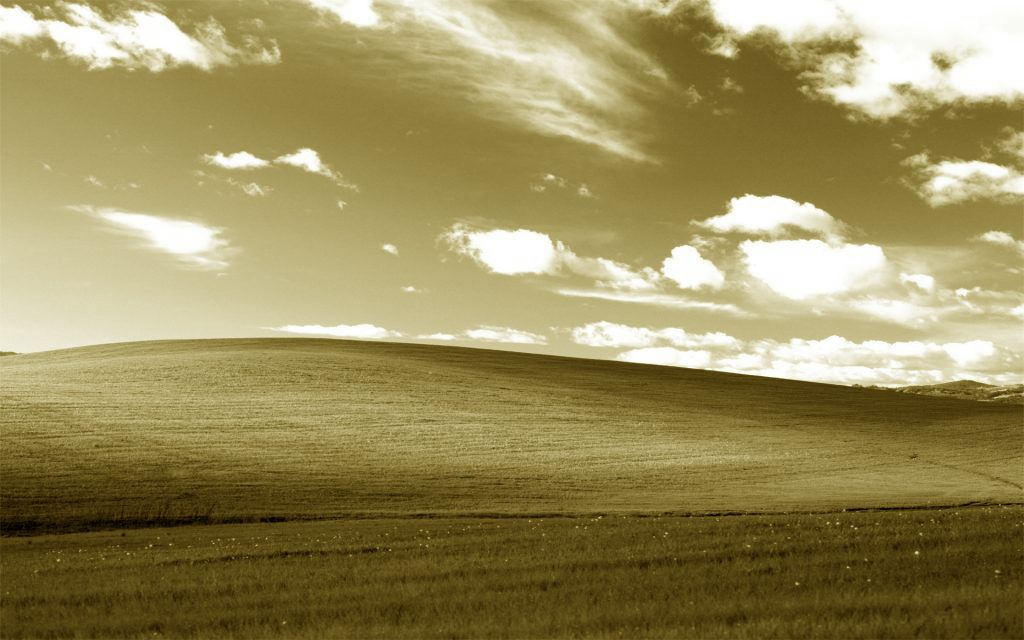
\includegraphics[width=\linewidth]{szepia.jpg}
        \caption{Részábra 1}
        \label{subfig1}
    \end{subfigure}
    \hfill
    \begin{subfigure}{0.45\textwidth}
        
\includegraphics[width=\linewidth]{szines.jpg}
        \caption{Részábra 2}
        \label{subfig2}
    \end{subfigure}
    \caption{Részábrák egy ábrán belül}
    \label{fig:main_figure}
\end{figure}

\subsection{i) Feliratok és elrendezés szépítése}
% 1i. feladat
\begin{figure}[h]
    \centering
    \begin{subfigure}{0.4\textwidth}
        \centering
        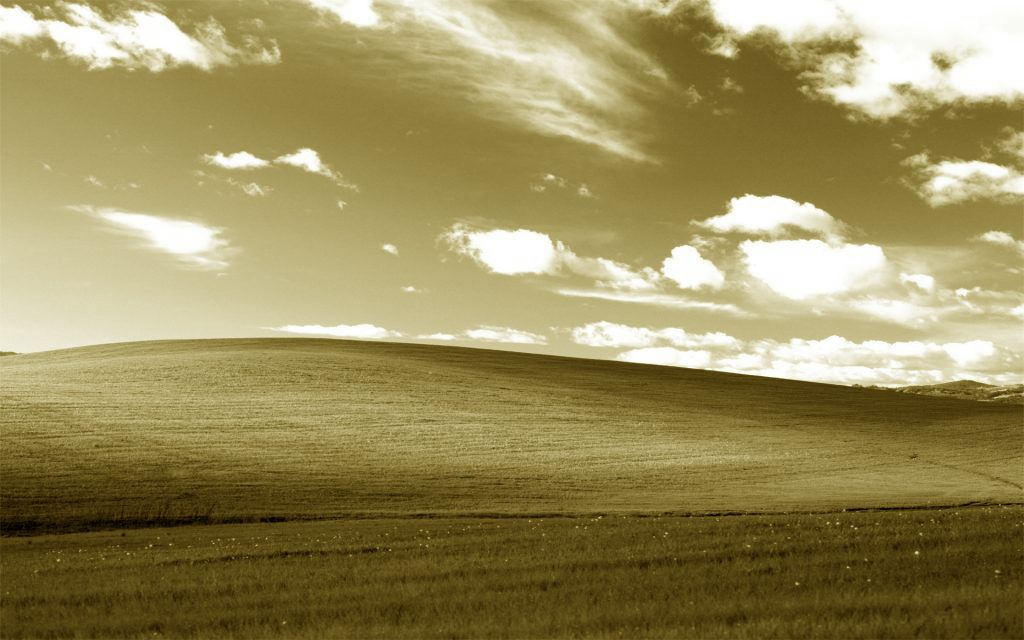
\includegraphics[width=\linewidth]{szepia.jpg}
        \caption{Részábra 1}
        \label{subfig1}
    \end{subfigure}\hfill
    \begin{subfigure}{0.4\textwidth}
        \centering
        
\includegraphics[width=\linewidth]{szines.jpg}
        \caption{Részábra 2}
        \label{subfig2}
    \end{subfigure}
    \caption{Két részábra középre igazítva és térköz beállítással}
    \label{fig:aligned_fig}
\end{figure}

Hivatkozás a fő ábrára: \ref{fig:main_figure}, részábrákra: \subref{subfig1} és \subref{subfig2}.

\newpage

\section{Táblázatok feladat}

\subsection{a) Első táblázat}
% 2a. feladat
\begin{table}[h]
    \centering
    \begin{tabular}{|p{30pt}|l|c|r|}
        \hline
        Cell 1 & Balra igazított & Középre & Jobbra igazított \\ \hline
        Tartalom 1 & Tartalom 2 & Tartalom 3 & Tartalom 4 \\ \hline
        Tartalom 5 & & Tartalom 7 & Tartalom 8 \\ \hline
        Tartalom 9 & Tartalom 10 & Tartalom 11 & Tartalom 12 \\ \hline
    \end{tabular}
    \caption{Első táblázat}
    \label{tab:table1}
\end{table}

\subsection{b) Színes táblázat (váltakozó sorok)}
% 2b. feladat
\begin{table}[h]
    \centering
    \rowcolors{1}{gray!20}{white}
    \begin{tabular}{|l|c|r|}
        \hline
        Sor 1 & Adat 1 & Adat 2 \\ \hline
        Sor 2 & Adat 1 & Adat 2 \\ \hline
        Sor 3 & Adat 1 & Adat 2 \\ \hline
    \end{tabular}
    \caption{Váltakozó színezésű táblázat}
\end{table}

\subsection{c) Táblázatok listázása}
% 2c. feladat
A táblázatok listáját a dokumentum elején találhatjuk.

\subsection{d) Cellák egyesítése táblázatban}
% 2d. feladat
\begin{table}[h]
    \centering
    \begin{tabular}{|l|c|r|}
        \hline
        Cellák egyesítése vízszintesen & \multicolumn{2}{|c|}{Egyesített cellák} \\ \hline
        Függőlegesen & \multirow{2}{*}{Egyesített} & Adat \\ \cline{3-3}
        & & Adat \\ \hline
    \end{tabular}
    \caption{Cellák egyesítése}
    \label{tab:merged}
\end{table}

\subsection{e) Táblázat úsztatása}
% 2e. feladat
\begin{wraptable}{r}{0.5\textwidth}
    \centering
    \begin{tabular}{|l|c|}
        \hline
        Adat 1 & Adat 2 \\ \hline
        Adat 3 & Adat 4 \\ \hline
    \end{tabular}
    \caption{Körbefuttatott táblázat}
\end{wraptable}

\newpage

\section{Verbatim feladat}

\subsection{a) Inline verbatim használata}
% 3a. feladat
Ez egy mondat \verb|\LaTeX| paranccsal benne.

\subsection{b) Verbatim környezet használata}
% 3b. feladat
\begin{verbatim}
\begin{enumerate}
    \item Első elem
    \item Második elem
\end{enumerate}
\end{verbatim}

\newpage

\section{Programkód 1 (Python)}

\subsection{a) Python kódrészlet beillesztése}
% 4a. feladat
\lstinputlisting{bin_ker.py}

\subsection{b-e) Programnyelv, tabulátorok, sorok számozása és keretezés}
% 4b-4e feladat
A Python kód automatikusan formázódik és sorszámozódik.

\newpage

\section{Programkód 2 (C)}

\subsection{a) C kódrészlet beillesztése fájlszerkezetben}
% 5a. feladat
\lstinputlisting{binsearch.c}

\newpage

% 6. feladat
% Új float környezetek definiálása
\newfloat{PythonCode}{htbp}{lop}
\floatname{PythonCode}{Python Kód}

\newfloat{CCode}{htbp}{loc}
\floatname{CCode}{C Kód}

\section{Float feladat}

\subsection{a) Python kód beillesztése}
\begin{PythonCode}[H]
    \caption{Példa Python kód}
    \lstinputlisting{bin_ker.py}
\end{PythonCode}

\subsection{b) C kód beillesztése}
\begin{CCode}[H]
    \caption{Példa C kód}
    \lstinputlisting[language=C]{binsearch.c}
\end{CCode}

\subsection{c) Caption a kódok fölött}
A fenti kódok esetén a caption a kódok fölött jelenik meg.

\subsection{d) Másolat a C kódrészletről}
\begin{CCode}[H]
    \caption{Második C kód példa (másik függvény)}
    \lstinputlisting[language=C]{binsearch.c} % A második függvény kódja
\end{CCode}

\newpage

\subsection{e) Programtípusok listázása}
A következő programtípusokat tartalmazza a dokumentum:
\begin{itemize}
    \item Python Kód
    \item C Kód
\end{itemize}


\end{document}
